\documentclass[11pt,a4paper]{article}
\usepackage[margin=1in]{geometry}
\usepackage{amsmath,amssymb,amsthm,mathtools}
\usepackage{booktabs}
\usepackage{tabularx}
\usepackage{graphicx}
\usepackage{lmodern}
\usepackage[T1]{fontenc}
\usepackage{microtype}
\usepackage[hidelinks]{hyperref}
\usepackage{enumitem}
\setlist{nosep,leftmargin=1.2em}

\newtheorem{theorem}{Theorem}[section]
\newtheorem{lemma}[theorem]{Lemma}
\newtheorem{proposition}[theorem]{Proposition}
\newtheorem{corollary}[theorem]{Corollary}
\theoremstyle{definition}
\newtheorem{definition}[theorem]{Definition}
\newtheorem{remark}[theorem]{Remark}
\newtheorem{conjecture}[theorem]{Conjecture}
\newtheorem{example}[theorem]{Example}

\newcommand{\T}{\textnormal{\textbf{[T]}}}
\newcommand{\V}{\textnormal{\textbf{[V]}}}
\newcommand{\Cc}{\textnormal{\textbf{[C]}}}
\newcommand{\Dd}{\textnormal{\textbf{[D]}}}
\newcommand{\Hh}{\textnormal{\textbf{[H]}}}
\newcommand{\Fr}{F}
\newcommand{\PP}{\Pi}
\newcommand{\QQ}{Q}
\newcommand{\df}{\mathrm{d}}
\newcommand{\Tr}{\operatorname{Tr}}
\newcommand{\R}{\mathbb{R}}
\newcommand{\C}{\mathbb{C}}
\newcommand{\norm}[1]{\lVert#1\rVert}
\newcommand{\abs}[1]{\lvert#1\rvert}
\newcommand{\ip}[2]{\langle#1,#2\rangle}
\newcommand{\Gap}{\gamma}
\newcommand{\shape}{\Sigma}
\newcommand{\lean}[1]{\texttt{#1}}
\newcommand{\gate}[1]{\texttt{#1}}

\title{\bfseries Gaps and Totals\\[2pt]
\large an operator-first theory of transport invariants,\\ with the shape sphere solved exactly}
\author{Jeromie Beasley}
\date{Draft --- \today}

\begin{document}
\maketitle

\begin{abstract}
Transport is usually described by the trajectories it produces. This paper describes it by what
survives: a family of admissible subspaces carried along a path, and the gap that decides what can
be resolved at the end of it. Two things follow, and both are theorems rather than slogans.
\emph{Gaps}: a transport invariant is stable to the extent that the gap across the
boundary of the cluster defining it is open. That principle is made quantitative here --- the corpus's own tip-and-tail
law states it, and what is added is how much each level gains. A rank-one projector buys no
stability at all, because in operator norm it moves at the same rate as its eigenvector.
The gain belongs to clusters, whose protection is the external gap. \emph{Totals}: the distance
map of $N$ bodies has a conserved total capacity, $\sum_{i<j}\lVert\nabla d_{ij}\rVert^2=N(N-2)$
for equal unit masses, so the shape only redistributes a total fixed by $N$. On the equal-mass three-body
shape sphere the redistribution is solved exactly: the squared singular values sum to $3$, their
product is $12A^2/(d_{12}^2d_{13}^2d_{23}^2)$, for the map to the distances the degeneracy at the equilateral shape is a linear
isotropic cone of slope $3$ with holonomy $-1$, the rank dropping exactly where the gap is
largest; for the map to the squared distances it is a quadratic fold with holonomy $+1$, and the
two statements are both true of their own operator. Every claim carries a grade, and the finite ones are machine-checked: 29 kernel-checked theorems, 79 gate
assertions, six deliberately false statements that the checker must reject.

\end{abstract}

\tableofcontents

\section{Introduction}\label{sec:intro}

\subsection{One idea, ten coats}

The operator-first transport programme that this paper belongs to is a series of preprints
\Cc{} around a single structure: a family of subspaces carried along a path, together with the
quantity that decides what can be resolved along the way. The series places that quantity in
different positions --- in the spectrum (Riesz projectors, exceptional points), between two
subspaces (principal angles, persistence), in the pseudospectrum (transient growth), at an
interface (refraction, Schur complements), or in the readout (numerator selection) --- and each
placement is a paper. What the series has not had is a statement of the structure that is
narrow enough to be wrong. This paper attempts one --- for three of its objects, and in a
different idiom: it uses the standard quantum geometric tensor and none of the programme's own
machinery (Dirac time, the vacuum-operator two-parameter family, connection energy). It is a
companion line, not a replacement for any part of the programme, and where it touches the
corpus's results it does so as an independent check.

\subsection{The thesis}

Two sentences, and the paper is their elaboration.

\begin{enumerate}[label=(\roman*)]
\item \textbf{Gaps.} A transport invariant is stable to the extent that the gap across
the boundary of the cluster defining it is open, and the relevant gap is never the one inside
the cluster.
\item \textbf{Totals.} A transport can forget almost every direction and still retain a constant;
for the distance map of $N$ bodies that constant is $N(N-2)$, and the shape only decides how it
is distributed.
\end{enumerate}

The first sentence is a correction of the series' ``hierarchy principle of structural
persistence'', which as stated is false at its first level. The second is a theorem the series
did not have, and it is a different statement from the per-shape spectral formula, not a
correction of it: that formula is about the map to squared distances and holds for its own
operator (Remark~\ref{rem:twomaps}).

\subsection{What is new here}

\begin{enumerate}[label=\textbf{C\arabic*.},leftmargin=2.2em]
\item \textbf{The redistribution theorem} (\S\ref{sec:redistribution}). The off-diagonal part of
a structural operator is traceless, vanishes if and only if the operator commutes with the
projector, and has the same Frobenius norm as the commutator. The algebra is elementary; the
point is that it makes ``redistribution'' and ``non-commutativity'' the same quantity, which the
series treats as two phenomena.

\item \textbf{The geometry is derived} (\S\ref{sec:geometry}). The quantum geometric tensor of a
projector family is $Q_{\mu\nu}=\Tr(\PP\partial_\mu\PP\partial_\nu\PP)$; its real part is a metric
because it is a squared norm of a block of $\dot\PP$, and the curvature is $-2\operatorname{Im}Q$
with $\abs{\omega}\le2\sqrt{g_{\mu\mu}g_{\nu\nu}}$. The object the series writes down,
$\Tr(\partial_\mu\PP\partial_\nu\PP)$, is real and is twice the metric; it cannot carry curvature.

\item \textbf{The hierarchy, quantified} (\S\ref{sec:hierarchy}). With constants: eigenvalues are
$1$-Lipschitz and unprotected; a rank-one projector moves at exactly the eigenvector's rate in
operator norm and $\sqrt2$ faster in Frobenius, so it protects nothing; a cluster projector is
protected by the external gap --- with the union gap in the denominator for a finite pair, and
constant $1$ in the infinitesimal form that the paper uses --- and its angle obeys a sharp
$\tan 2\Theta$ bound when the perturbation is off-diagonal and the cluster is a separated simple
eigenvalue; the $\pi/2$ that circulates in the
literature is the constant of the angle bound, attained at the edge of the stable range;
integers are locally constant. The exceptional point is invisible to the cluster and fatal to the basis.

\item \textbf{The capacity sum rule} (\S\ref{sec:totals}). $\sum_{i<j}\norm{\nabla d_{ij}}^2
=(N-1)\sum_i1/m_i-\sum_{i<j}d_{ij}^2$, hence $N(N-2)$ for equal unit masses, for every
configuration. The total is combinatorial; the distribution is the shape.

\item \textbf{The shape sphere, solved} (\S\ref{sec:shape}). $\sigma_1^2+\sigma_2^2=3$,
$\det M^*M=12A^2/(d_{12}^2d_{13}^2d_{23}^2)$ with maximum $9/4$ exactly at the equilateral shapes
and zero exactly on the collinear locus, a linear isotropic cone of slope $3$, rank drop where the
gap is largest, and holonomy $-1$. Mass symmetry breaking does not create the cone and does not
tilt it: it moves the two optic points off the equilateral shapes by $\varepsilon^2/9$ and makes
the cone elliptic.

\item \textbf{Refraction, demoted} (\S\ref{sec:refraction}). $\rho_1\sin^2\theta_1=\rho_2\sin^2
\theta_2$ is Snell's law for the conformal metric $\rho g$. The theorem is about geodesics; the
claim that a physical medium is conformal with factor $\rho$ is a hypothesis, and saying which is
which is the point.
\end{enumerate}

\subsection{What is not claimed}

No physical system is modelled here, and \S\ref{sec:scope} says so at the level of individual
claims: the covariance-data reproduction is a consistency check on published data and not
evidence for the framework; the cosmological reading is circular as stated and is not used; the
psychophysical reading is an interpretation without a theorem. The paper also does not claim that
the framework is new mathematics --- the algebra of \S\S\ref{sec:redistribution}--\ref{sec:geometry}
is elementary and the classical inputs of \S\ref{sec:hierarchy} are classical. What is new is the
assemblage, the constants of \S\ref{sec:hierarchy}, and the two exact results of
\S\S\ref{sec:totals}--\ref{sec:shape}. Several remarks record corrections; the reader should know
that some of them correct earlier drafts of \emph{this} paper rather than the corpus.

\subsection{How to read it}

Every statement carries a grade --- \T\ proved, \V\ machine-verified with the file and residual
named, \Cc\ cited, \Dd\ data, \Hh\ hypothesis --- and where a chain mixes grades the weakest link
is named in the sentence that draws the conclusion (\S\ref{sec:setting}). The paper is written to
be checked rather than believed: \S\ref{sec:refute} lists, for each claim, the cheapest
observation that would falsify it, and Appendix~\ref{app:repro} gives the commands that
re-run everything.

\subsection{Roadmap}

\S\ref{sec:setting} fixes notation and one symbol per concept. \S\ref{sec:redistribution} proves
the redistribution theorem, \S\ref{sec:geometry} derives the metric and curvature from it,
\S\ref{sec:hierarchy} states the hierarchy with its constants, crediting the corpus's own
tip-and-tail law, and records where earlier drafts of this paper were wrong.
\S\ref{sec:totals} proves the sum rule, \S\ref{sec:shape} solves the shape sphere,
\S\ref{sec:refraction} disposes of the refraction law. \S\S\ref{sec:scope}--\ref{sec:open} state
the scope, the refutations and the open problems; the appendices carry the ledger, the
reproduction instructions and the classical inputs.

\section{Setting, notation, and the rules of evidence}\label{sec:setting}

\subsection{The transport datum}

Throughout, $H$ is a finite-dimensional real or complex Hilbert space of dimension $n$,
$\ip{\cdot}{\cdot}$ its inner product, $\norm{\cdot}$ the operator norm and
$\norm{X}_F^2=\Tr(X^*X)$ the Frobenius (Hilbert--Schmidt) norm. $\PP$ always denotes an
\emph{orthogonal} projector, $\PP^*=\PP$, $\PP^2=\PP$, and $\QQ:=1-\PP$. $\Tr$ is the trace.
A \emph{transport datum} is a triple
\[
   \bigl(t\mapsto A(t),\ \PP(t),\ \Gap(t)\bigr),
\]
where $A(t)$ is a $\C^1$ family of self-adjoint operators, $\PP(t)$ is the orthogonal projector
onto a \emph{spectral cluster} $\shape(t)\subset\operatorname{spec}A(t)$, and $\Gap(t)>0$ is the
distance from $\shape(t)$ to the rest of the spectrum. The cluster is the \emph{admissible
subspace}; the gap $\Gap$ is the only quantity in the theory that is not derived from $A$ and
$\PP$ themselves.

\begin{remark}[Why a cluster and not an eigenvalue]\label{rem:cluster}
The theory is stated for clusters even where a single eigenvalue would do, because the two
behave differently under deformation (\S\ref{sec:hierarchy}). A single-eigenvalue cluster and a
rank-one projector carry the same information, and \S\ref{sec:hierarchy} shows that the
projector gains nothing; the gain appears only for clusters of two or more eigenvalues.
\end{remark}

\subsection{Invariants, and the one symbol per concept rule}

The corpus this paper belongs to has three different objects called $C$: a transport capacity,
a persistence overlap, and a boundary census. One symbol per concept, from here on.

\begin{center}
\small
\begin{tabularx}{\textwidth}{@{}l l >{\raggedright\arraybackslash}X@{}}
\toprule
symbol & object & defined in \\
\midrule
$\Omega$ & structural operator, a self-adjoint field & \S\ref{sec:redistribution} \\
$\Fr(\Omega,\PP)$ & redistribution operator $\PP\Omega\QQ+\QQ\Omega\PP$ & \S\ref{sec:redistribution} \\
$\pi(\PP_1,\PP_2)$ & persistence $\Tr(\PP_1\PP_2)$ & \S\ref{sec:setting} \\
$\rho$ & rigidity $\sigma_{\min}^{-2}$ & \S\ref{sec:shape} \\
$Q_{\mu\nu}$ & quantum geometric tensor & \S\ref{sec:geometry} \\
$g_{\mu\nu}$ & quantum metric $\operatorname{Re}Q_{\mu\nu}$ & \S\ref{sec:geometry} \\
$\omega_{\mu\nu}$ & curvature $-2\operatorname{Im}Q_{\mu\nu}$ & \S\ref{sec:geometry} \\
$\sigma_i$ & singular values of the transport differential & \S\ref{sec:shape} \\
$\kappa$ & cone slope & \S\ref{sec:shape} \\
\bottomrule
\end{tabularx}
\end{center}

The persistence of two projectors is the one invariant that needs no gap:
\begin{equation}\label{eq:persistence}
   \pi(\PP_1,\PP_2):=\Tr(\PP_1\PP_2)=\norm{\PP_2\PP_1}_F^2\ \in[0,\min(k_1,k_2)],
\end{equation}
which is \T\ and kernel-checked,\footnote{\lean{EmergentTransport/Basic.lean}:
\lean{persistence\_frobenius}, \lean{persistence\_nonneg}, and at rank one with value
$(u\cdot v)^2=\cos^2\theta$, \lean{persistence\_rank\_one}.} with the rank-one value
$(u\cdot v)^2=\cos^2\theta$; the principal-angle form $\sum_i\cos^2\theta_i$ for higher rank is
classical \Cc{} and is not used below.

\subsection{The five grades, and the weakest-link rule}

Every statement carries one of
\begin{center}
\begin{tabular}{@{}ll@{}}
\toprule
grade & meaning \\
\midrule
\T & proved in this paper (or kernel-checked, marked \lean{name}) \\
\V & verified by a named gate or script, with the file and the measured residual \\
\Cc & cited, with the hypotheses under which it holds stated \\
\Dd & data reported under a stated protocol, not measured here \\
\Hh & hypothesis or interpretation, not established \\
\bottomrule
\end{tabular}
\end{center}
Where a chain of reasoning mixes grades, the weakest link is named in the sentence that states
the conclusion. This is the corpus's own convention and it is the reason the paper can be
audited rather than believed.

\subsection{What is not assumed}

No metric on the space of parameters is assumed: the metric of \S\ref{sec:geometry} is
\emph{derived} from the projector family, and the statement that it is a metric is a theorem
(\S\ref{sec:geometry}), not a definition. No genericity is assumed except where stated
(simple eigenvalues, non-degeneracy of a gap). No smoothness beyond $\C^1$ is assumed except
where derivatives of higher order appear, and there it is stated. No physical system is
assumed; \S\ref{sec:scope} says exactly what is and is not claimed about the physical readings
the corpus attaches to the framework.

\section{Redistribution: what moves between blocks}\label{sec:redistribution}

Fix an orthogonal projector $\PP$ and write $\QQ=1-\PP$. Every operator decomposes into four
blocks, and the two off-diagonal ones are the only ones that can carry anything between the
admissible subspace and its complement.

\begin{definition}[Redistribution operator]\label{def:F}
For $\Omega\in\operatorname{End}(H)$,
\begin{equation}\label{eq:F}
   \Fr(\Omega,\PP):=\PP\Omega\QQ+\QQ\Omega\PP .
\end{equation}
\end{definition}

\begin{lemma}[Block decomposition]\label{lem:blocks}
For every $\Omega$, $\ \Omega=\PP\Omega\PP+\PP\Omega\QQ+\QQ\Omega\PP+\QQ\Omega\QQ$, and the two
off-diagonal blocks of $\Fr(\Omega,\PP)$ are the off-diagonal blocks of $\Omega$:
\[
   \PP\,\Fr(\Omega,\PP)\,\QQ=\PP\Omega\QQ,\qquad
   \QQ\,\Fr(\Omega,\PP)\,\PP=\QQ\Omega\PP .
\]
\T\ Kernel-checked: \lean{block\_decomposition}, \lean{redistribution\_block12},
\lean{redistribution\_block21} (\lean{EmergentTransport/GapsAndTotals.lean}).
\end{lemma}

\begin{proof}
$\PP\Omega\PP+\PP\Omega\QQ=\PP\Omega(\PP+\QQ)=\PP\Omega$ and likewise for $\QQ$; adding gives
$\Omega$. For the blocks, $\PP\Fr\QQ=\PP(\PP\Omega\QQ+\QQ\Omega\PP)\QQ=\PP\Omega\QQ\,\QQ+\PP\QQ\,\Omega\PP\QQ=\PP\Omega\QQ$,
using $\PP\QQ=0$ and $\QQ^2=\QQ$. The other block is the same computation with $\PP$ and $\QQ$
interchanged.
\end{proof}

So $\Fr$ is exactly the off-diagonal part, and $0=\Fr$ is exactly the statement that $\Omega$ is
block-diagonal.

\begin{theorem}[Redistribution is traceless]\label{thm:traceless}
For every $\Omega$ and every idempotent $\PP$ (orthogonality is not needed here),
$\Tr\Fr(\Omega,\PP)=0$.
\T\ Kernel-checked: \lean{redistribution\_traceless}.
\end{theorem}

\begin{proof}
$\Tr(\PP\Omega\QQ)=\Tr(\Omega\QQ\PP)=0$ by cyclicity and $\QQ\PP=0$; likewise
$\Tr(\QQ\Omega\PP)=0$.
\end{proof}

\begin{theorem}[Compatibility]\label{thm:compat}
$\Fr(\Omega,\PP)=0$ if and only if $\Omega\PP=\PP\Omega$. Neither self-adjointness of $\Omega$
nor orthogonality of $\PP$ is used.
\T\ Kernel-checked: \lean{redistribution\_zero\_iff\_commute}.
\end{theorem}

\begin{proof}
($\Leftarrow$) If $\Omega\PP=\PP\Omega$ then $\PP\Omega\QQ=\PP(\Omega\QQ)=\PP(\QQ\Omega)=\PP\QQ\Omega=0$
and $\QQ\Omega\PP=(\QQ\Omega)\PP=(\Omega\QQ)\PP=\Omega(\QQ\PP)=0$.
($\Rightarrow$) If $\Fr=0$ then by Lemma~\ref{lem:blocks} both $\PP\Omega\QQ$ and $\QQ\Omega\PP$
vanish, so $\Omega=\PP\Omega\PP+\QQ\Omega\QQ$ and therefore
$\Omega\PP=\PP\Omega\PP=\PP\Omega$.
\end{proof}

The next result is the quantitative one: the \emph{size} of the movement between blocks equals
the size of the failure to commute.

\begin{theorem}[Norm identity]\label{thm:norm}
Let $\Omega$ be self-adjoint and $\PP$ an orthogonal projector. Then
\begin{equation}\label{eq:norm}
   \norm{\Fr(\Omega,\PP)}_F^2 \;=\; 2\,\norm{\PP\Omega\QQ}_F^2 \;=\; \norm{[\Omega,\PP]}_F^2 ,
   \qquad\text{and}\qquad \tfrac12\norm{[\Omega,\PP]}_F^2=\norm{\PP\Omega\QQ}_F^2 .
\end{equation}
Moreover $[\Omega,\PP]$ is skew: $[\Omega,\PP]^*=-[\Omega,\PP]$.
\T\ Kernel-checked: \lean{redistribution\_norm}, \lean{commutator\_skew},
\lean{half\_commutator\_norm}.
\end{theorem}

\begin{proof}
Put $A=\PP\Omega\QQ$ and $B=\QQ\Omega\PP$. Since $\Omega^*=\Omega$ and $\PP^*=\PP$,
$B=A^*$. Since $\QQ\PP=0$, $A^2=\PP\Omega\QQ\PP\Omega\QQ=0$, and likewise $B^2=0$.
Then $\Fr=A+B$, $\Fr^*=\Fr$, and
\[
   \norm{\Fr}_F^2=\Tr\bigl((A+A^*)^2\bigr)=2\norm{A}_F^2+2\operatorname{Re}\Tr(A^2)=2\norm{A}_F^2 .
\]
For the commutator, $[\Omega,\PP]=\Omega\PP-\PP\Omega=(\QQ\Omega\PP+\PP\Omega\PP)-(\PP\Omega\PP+\PP\Omega\QQ)=B-A=A^*-A$,
so $\norm{[\Omega,\PP]}_F^2=\Tr\bigl((A^*-A)(A-A^*)\bigr)=2\norm{A}_F^2-2\operatorname{Re}\Tr(A^2)=2\norm{A}_F^2$.
Skewness is immediate from $\Omega^*=\Omega$, $\PP^*=\PP$.
\end{proof}

\begin{remark}[A correction, recorded]\label{rem:corrected-chain}
An earlier formulation of this section chained the equalities as
$\norm{\Fr}^2=2\norm{\PP\Omega\QQ}^2=\tfrac12\norm{[\Omega,\PP]}^2$. That is false: the last
two terms differ by a factor $4$. The counterexample is $\PP=\operatorname{diag}(1,0)$,
$\Omega=\sigma_1$, for which $\norm{\Fr}_F^2=2$, $\norm{\PP\Omega\QQ}_F^2=1$ and
$\norm{[\Omega,\PP]}_F^2=2$, so $\tfrac12\norm{[\Omega,\PP]}_F^2=1\neq 2$. The correct chain is
\eqref{eq:norm}: $\Fr$ and the commutator have \emph{the same} squared norm, and the half-factor
belongs to the second identity, where it converts a squared commutator into a squared metric
block. This is the form proved in the kernel and the form used in \S\ref{sec:geometry}.
\end{remark}

\begin{example}[Non-normal $\Omega$: traceless but not balanced]\label{ex:nonnormal}
The first conclusion survives non-normality and the second does not. Take
$\Omega=\left(\begin{smallmatrix}0&1\\0&0\end{smallmatrix}\right)$, $\PP=\operatorname{diag}(1,0)$. Then
$\Fr(\Omega,\PP)=\left(\begin{smallmatrix}0&1\\0&0\end{smallmatrix}\right)$, so $\Tr\Fr=0$ and
$\norm{\Fr}_F^2=1=\norm{\PP\Omega\QQ}_F^2$; the factor $2$ of \eqref{eq:norm} is absent because
$\Omega$ is not self-adjoint ($\Omega\Omega^*\neq\Omega^*\Omega$). \V\ \lean{FalseControls/norm\_needs\_selfadjoint.lean}, which the verification requires
to \emph{fail}.
\end{example}

\begin{remark}[What the section says, in one sentence]
A transport can move structure across an interface exactly to the extent that the structural
operator fails to commute with the projector, and the amount moved is the whole of that
failure --- there is no third thing.
\end{remark}

\section{The geometry is derived, not assumed}\label{sec:geometry}

Let $\PP(x)$ be a $\C^1$ family of orthogonal projectors of constant rank $k$, parametrised by
$x=(x^1,\dots,x^m)$ in an open set. Write $\partial_\mu=\partial/\partial x^\mu$.

\begin{definition}[Quantum geometric tensor of a projector family]\label{def:qgt}
\begin{equation}\label{eq:qgt}
   Q_{\mu\nu}(x):=\Tr\bigl(\PP\,\partial_\mu\PP\,\partial_\nu\PP\bigr),\qquad
   g_{\mu\nu}:=\operatorname{Re}Q_{\mu\nu},\qquad
   \omega_{\mu\nu}:=-2\operatorname{Im}Q_{\mu\nu}.
\end{equation}
\end{definition}

The placement of $\PP$ matters and is the point of the next remark.

\begin{theorem}[$Q$ is a Hermitian tensor and $g$ is a metric]\label{thm:qgt}
$Q$ is Hermitian, $g$ is symmetric and positive semidefinite, and for a single parameter with
variation $\dot\PP$,
\begin{equation}\label{eq:metric-norm}
   g(\dot\PP,\dot\PP)=\norm{\PP\dot\PP\QQ}_F^2=\tfrac12\norm{\dot\PP}_F^2=\tfrac12\Tr(\dot\PP^2).
\end{equation}
The identity $g_\PP(V,V)=\tfrac12\Tr(V^2)$ is the June paper's \Cc{} \cite{corpus}, where
the metric is defined that way; what is added here is the derivation, which makes it the
special case of the redistribution theorem: $\dot\PP=\PP\dot\PP\QQ+\QQ\dot\PP\PP$
(differentiate $\PP^2=\PP$), so Theorem~\ref{thm:norm} applied to $\Omega=\dot\PP$ gives
$\norm{\PP\dot\PP\QQ}_F^2=\tfrac12\norm{\dot\PP}_F^2$. \T\ for the derivation, \Cc\ for the
identity; the kernel checks both halves (\lean{redistribution\_norm},
\lean{half\_commutator\_norm}).
\end{theorem}

\begin{proof}
Hermiticity: $\overline{Q_{\nu\mu}}=\overline{\Tr(\PP\partial_\nu\PP\partial_\mu\PP)}=\Tr\bigl((\PP\partial_\nu\PP\partial_\mu\PP)^*\bigr)=\Tr(\PP\partial_\mu\PP\partial_\nu\PP)=Q_{\mu\nu}$.
Positivity: put $Z_\mu:=\QQ\partial_\mu\PP\,\PP$. Since $\partial_\mu\PP=\PP\partial_\mu\PP\QQ+\QQ\partial_\mu\PP\PP$,
$\Tr(\PP\partial_\mu\PP\partial_\nu\PP)=\Tr(\PP\partial_\mu\PP\,\QQ\,\partial_\nu\PP)=\Tr(Z_\mu^*Z_\nu)$,
so $Q_{\mu\nu}=\ip{Z_\mu}{Z_\nu}_F$ and $g_{\mu\mu}=\norm{Z_\mu}_F^2\ge0$. Equation
\eqref{eq:metric-norm} is the special case $\mu=\nu$ together with Theorem~\ref{thm:norm}.
\end{proof}

\begin{remark}[A second correction: the tensor must carry the projector]\label{rem:qgt-correction}
An earlier formulation used $Q^\circ_{\mu\nu}=\Tr(\partial_\mu\PP\,\partial_\nu\PP)$ as the
quantum geometric tensor. That object is real: $\partial_\mu\PP$ is self-adjoint, so
$(\partial_\mu\PP\partial_\nu\PP)^*=\partial_\nu\PP\partial_\mu\PP$ and $\Tr$ of the product is
real, hence $\operatorname{Im}Q^\circ=0$ identically and $Q^\circ$ cannot carry curvature. What
it is, by Theorem~\ref{thm:qgt}, is twice the metric: $Q^\circ=2g$. The corrected tensor $Q$ of
\eqref{eq:qgt} has a genuine imaginary part, and it is the corpus's own form: its later paper
\Cc{} \cite{iqgt} writes the intrinsic tensor as $Q_{\PP}(V,W)=\Tr(\PP VW)$, which is
\eqref{eq:qgt} for $V=\partial_\mu\PP$, $W=\partial_\nu\PP$; the object $Q^\circ$ was not in fact
a form the corpus ever used --- the June paper states $Q_\PP(V,W)=\Tr(\PP VW)$ already --- so
this remark corrects an earlier draft of \emph{this} paper, not the corpus. \V\ Both facts are measured in
\gate{results/swarm/check\_D2\_m7.py} (literal imaginary part exactly zero; nonzero curvature
$0.358678$): two independent reports found the same error, which is why it is recorded here
rather than quietly repaired.
\end{remark}

\begin{theorem}[Curvature and its periods]\label{thm:curv}
For a $\C^2$ family, $\omega=\tfrac12\omega_{\mu\nu}\df x^\mu\wedge\df x^\nu$ is closed,
$\df\omega=0$. For a closed oriented surface $\shape$ and rank $k=1$,
$\frac1{2\pi}\int_\shape\omega\in\mathbb{Z}$; for higher rank the trace of the curvature is
likewise integral (Chern--Weil). \T\ closedness, from $\PP^2=\PP$ and the symmetry of mixed
partials; the integrality is classical \Cc{} (Chern--Weil theory; for the rank-one case the
Berry phase about a cone is $\pi$ per unit winding, \S\ref{sec:hierarchy}).
\end{theorem}

\begin{theorem}[Metric--curvature bound]\label{thm:bound}
For every rank $k$ and every pair of tangent directions $V,W$,
\begin{equation}\label{eq:bound}
   \abs{\omega(V,W)}\;\le\;2\sqrt{g(V,V)g(W,W)-g(V,W)^{2}}\;\le\;2\sqrt{g(V,V)g(W,W)} ,
   \qquad\text{and}\qquad \abs{\operatorname{Im}Q(V,W)}\le\tfrac12\abs{\omega(V,W)} .
\end{equation}
All three are Gram-determinant inequalities for the pair $Z_V,Z_W$ of
Theorem~\ref{thm:qgt}: $\abs{Q(V,W)}^2=g(V,W)^2+\tfrac14\omega(V,W)^2$ and
$g(V,V)g(W,W)\ge\abs{Q(V,W)}^2$. The first is sharp, with equality exactly when $V,W$ are
linearly dependent over $\C$; the second drops the Gram term and is sharp only when $g(V,W)=0$.
\T\ (Cauchy--Schwarz and the Gram determinant). Sharpness: \V\
\gate{results/swarm/check\_D3\_m1.py}.
\end{theorem}

\begin{remark}[The sharp form is the corpus's; an earlier draft of this paper was weaker]
\label{rem:factor2}
Theorem 12 of the June paper \Cc{} \cite{corpus} states
$\abs{\Omega_\PP(V,W)}\le2\sqrt{g_\PP(V,V)g_\PP(W,W)-g_\PP(V,W)^2}$, which with
$\Omega_\PP=2\operatorname{Im}Q=\omega$ is the first inequality of \eqref{eq:bound} --- the sharp
Gram-determinant form, valid for every rank because a Gram determinant does not see the rank.
An earlier draft of this paper offered $\abs{\omega}\le2\sqrt{g(V,V)g(W,W)}$ as a correction of
that bound. It is not one: the second inequality of \eqref{eq:bound} is the first with the Gram
term discarded, so the corpus's statement is the stronger of the two and this paper's was the
weaker. What survives of the earlier point is only that the constant $2$ belongs to the
\emph{curvature} and the constant $1$ to $\operatorname{Im}Q$ in the normalisation of
\eqref{eq:qgt} where $\omega=-2\operatorname{Im}Q$; in the corpus's normalisation
$Q=g+\tfrac{i}{2}\Omega$ the same statement reads $\abs{\Omega}\le2\sqrt{\cdot}$ and
$\abs{\operatorname{Im}Q}\le\sqrt{\cdot}$, which is the same pair of constants.
\end{remark}


\begin{remark}[What the section says, in one sentence]
The metric and the curvature are the symmetric and antisymmetric parts of one derived object,
the tensor $Q$, and the metric is not an input but a squared norm of a block of $\dot\PP$ ---
which is why \S\ref{sec:redistribution} had to come first.
\end{remark}

\section{The gap hierarchy: what is protected, and by what}\label{sec:hierarchy}

The corpus states a ``hierarchy principle of structural persistence'': individual eigenvectors
are fragile, projectors are stabler, global invariants are stabler still, and a transport
should therefore be described by its projectors. Its later paper \Cc{} \cite{iqgt}, \S10.2
(``the tip and the tail), already states the law that makes this precise: a single
eigenvector's gap is the distance to its nearest neighbour, while the cluster projector's is
the distance from the cluster to the rest of the spectrum, so the two are governed by
different gaps and the subspace inherits the stability of the outer one. This section does
not re-derive that principle. It adds the constants: which rate, in which norm, with which
finite-pair denominator, and how much a rank-one projector gains --- nothing.

\subsection{Levels 0 and 2: eigenvalues and cluster projectors}

\begin{theorem}[Weyl]\label{thm:weyl}
Let $A,A'$ be self-adjoint with eigenvalues ordered increasingly. Then for every $i$,
$\abs{\lambda_i(A')-\lambda_i(A)}\le\norm{A'-A}$.
\Cc\ (Weyl). The constant $1$ is sharp: $A=\operatorname{diag}(0,\gamma)$,
$A'=A+\epsilon\,\sigma_1$ moves the eigenvalues by $\pm\epsilon$ to first order.
\end{theorem}

Eigenvalues therefore have no protection at all: any perturbation moves them, and at a crossing
they lose their identity. Projectors are different, and the difference is the gap.

\begin{theorem}[Projector stability: finite bound and its infinitesimal form]\label{thm:riesz}
Let $A,A'$ be self-adjoint on $\C^n$, let $\shape\subset\operatorname{spec}A$ be a spectral
cluster --- \emph{any} cluster, including one with spectrum on both sides of it --- and put
$\Gap:=\operatorname{dist}(\shape,\operatorname{spec}A\setminus\shape)>0$,
$\delta:=\norm{A-A'}$. Let $\PP,\PP'$ be the orthogonal projectors onto the cluster and onto the
part of $\operatorname{spec}A'$ enclosed by a fixed contour separating $\shape$ from the rest,
with $\delta<\Gap/2$ so that the count cannot change (Weyl). Then
\begin{enumerate}[label=(\alph*)]
\item \textbf{(finite pair)} $\norm{\PP-\PP'}\le\delta/(\Gap-\delta)$\label{eq:prb}. The
denominator is the \emph{union} gap: $\Gap-\delta\le\operatorname{dist}(\shape,
\operatorname{spec}A'\setminus\shape')$. In particular $\norm{\PP-\PP'}\le2\delta/\Gap$ on the
stable range, and the ratio $\norm{\PP-\PP'}/(\delta/\Gap)$ can exceed $1$: an adversarial search
reaches $1.078$ at $\delta/\Gap=0.346$ (\V, gate \gate{g04\_projector\_constant}).
\item \textbf{(infinitesimal)} along a $\C^1$ path $t\mapsto A(t)$ whose gap is at least $\Gap$,
\begin{equation}\label{eq:deriv}
   \norm{\dot\PP}\le\norm{\dot A}/\Gap ,
\end{equation}
and the constant $1$ is sharp: the family $A(t)=R(2t)\operatorname{diag}(1,-1)R(-2t)$ attains
it. This is the form used everywhere below; the finite-pair bound (a) is \emph{not} the
infinitesimal one with $\delta$ replaced by $\norm{\dot A}$.
\item \textbf{(angle)} for $\Theta:=\arcsin\norm{\PP-\PP'}\in[0,\pi/2]$,
$\Theta\le\arcsin\bigl(\delta/(\Gap-\delta)\bigr)$. Since $\delta/(\Gap-\delta)$ increases from
$0$ to $1$ across the stable range, the angle bound increases from $0$ to $\pi/2$ and
\emph{attains} $\pi/2$ at its endpoint $\delta=\Gap/2$, where the count of the cluster is about
to change. So $\pi/2$ is the exact constant of the angle bound on the closure of the stable
range, \emph{in the class of perturbations of arbitrary form} --- which is where it belongs, and
not in (a) or (b). Restricting the class sharpens it; see Remark~\ref{rem:tan}. The literature
states the estimate in this angle form: Albeverio and Motovilov \Cc{} prove
$\arcsin\norm{\PP-\QQ}\le M(\norm{V}/\Gap)$ for $\norm{V}<\Gap/2$, and their bound is strong
enough to \emph{ensure} the acute-angle case for $\norm{V}<c\,\Gap$ with
$c=0.454169\ldots<1/2$. That is a sufficient condition, and it says nothing about what
happens above $c\,\Gap$; in particular it does not assert that acuteness fails there. What
(c) supplies is the complementary information: the bound\'s own value tends to $\pi/2$ as
$\delta\uparrow\Gap/2$, so $\pi/2$ is the exact supremum of the angle bound over the stable
range. We do not claim that the bound is attained at $\delta=\Gap/2$ by an actual pair, and
an earlier draft of this paper incorrectly reported the threshold $c$ as evidence that it was.
\end{enumerate}
\Cc\ for (a): the Davis--Kahan $\sin\theta$ theorem in its union-gap form is imported, not
re-proved. \T\ for (b), which follows from (a) applied to the pair $(A(t),A(t+h))$ with
$\delta=\norm{\dot A}h$ and $\Gap-\delta\to\Gap$, divided by $h$; and for (c), which is
monotonicity of $\arcsin$. \V\ Sharpness of (b), and the failure of the constant-$1$ form of
(a): gate \gate{g04\_projector\_constant}.
\end{theorem}

\begin{remark}[A correction, and a correction of the correction]\label{rem:piover2}
This paper first quoted, as \Cc, a constant $\pi/2$ for the general (two-sided) case and $1$ for
the ordered case. Drafting the proof showed that the assertion ``$\norm{\PP-\PP'}\le
\delta/\Gap$ with constant $1$'' is \emph{false} in the normalization used here --- a targeted
search produces $\norm{\PP-\PP'}=0.3735$ against $\delta=0.3465$ --- because Davis--Kahan's
denominator is the union gap $\Gap-\delta$, not $\Gap$. Both errors are recorded rather than
replaced: the $\pi/2$ belongs to the angle bound, and the constant $1$ belongs to the
\emph{derivative}, which is what the hierarchy table uses. Whether the finite-pair bound improves for an ordered
cluster, and in which term, is not something we needed and do not claim.
\end{remark}

\begin{theorem}[Rank one, line-separated: the sharp off-diagonal bound]\label{thm:tan2}
Let $A$ be self-adjoint with a simple eigenvalue $a$ and unit eigenvector $u$, and suppose every
other eigenvalue of $A$ lies at least $d>0$ \emph{above} $a$. Let $V$ be self-adjoint and
\emph{off-diagonal} with respect to $H=\operatorname{span}u\oplus u^\perp$, put
$\delta:=\norm V$, and let $\nu$ be the eigenvector of $A+V$ for the eigenvalue near $a$. With
$\Theta$ the angle between the two lines,
\begin{equation}\label{eq:tan2}
   \abs{\tan 2\Theta}\le\frac{2\delta}{d},
   \qquad\text{hence}\qquad
   \tan\Theta\le\frac{\sqrt{d^{2}+4\delta^{2}}-d}{2\delta}<\frac{\delta}{d}\quad(\delta>0).
\end{equation}
Both inequalities are sharp: for $A=\operatorname{diag}(a+d,a)$ and $V=\delta\sigma_1$ one has
$\tan\Theta=\delta\big/\bigl(d/2+\sqrt{d^{2}/4+\delta^{2}}\bigr)$ and
$\abs{\tan 2\Theta}=2\delta/d$ \emph{exactly}, for every $\delta<d/2$.
\T\ Proof below; \V\ gate \gate{g06\_projector\_tan2} (12 assertions).
\end{theorem}

\begin{proof}
Write $\nu=\cos\Theta\,u+\sin\Theta\,w$ with $\norm w=1$, $w\perp u$, and put
$b:=\ip{Aw}{w}$, $\mu:=\ip{u}{Vw}=\ip{Vu}{w}$. Because $Au=au$, $Aw\perp u$, $Vu\perp u$ and
$Vw\perp w$ (the last two by off-diagonality), the eigenvalue equation $(A+V)\nu=\lambda\nu$ has
exactly two scalar consequences,
\[
   (\lambda-a)\cos\Theta=\mu\sin\Theta,\qquad
   (\lambda-b)\sin\Theta=\mu\cos\Theta .
\]
Dividing the first by $\cos\Theta$ and the second by $\sin\Theta$ and subtracting,
$b-a=\mu(\tan\Theta-\cot\Theta)=-2\mu/\tan 2\Theta$, so
$\abs{\tan 2\Theta}=2\abs\mu/\abs{b-a}$. Now $\abs\mu=\abs{\ip{Vu}{w}}\le\norm{Vu}\le\delta$,
and $b$, being a numerical-range point of the compression of $A$ to $u^\perp$, lies in the convex
hull of the rest of the spectrum, every point of which exceeds $a$ by at least $d$; hence
$b-a\ge d$. This gives \eqref{eq:tan2}'s first bound, and the second follows by solving
$2t/(1-t^{2})\le2\delta/d$ for $t=\tan\Theta<1$.
\end{proof}

\begin{remark}[Why line separation cannot be dropped, and what the convex-hull hypothesis adds]
\label{rem:numerical-range}
The proof uses $b-a\ge d$, and that can fail while $\operatorname{dist}(a,\operatorname{spec}A
\setminus\{a\})=d$ still holds: if the rest of the spectrum straddles $a$, the convex hull of the
rest contains $a$, the compression's numerical range can put $b$ at $a$, and the bound breaks ---
gate \gate{g06\_projector\_tan2}(d) exhibits a violation by $1.21$. So \emph{line separation} is
the hypothesis this argument needs, and it is weaker than what the literature's convex-hull
condition is for: that condition is what lets the argument be run for clusters of rank $k\ge2$,
where the scalar reduction below no longer closes because $\Theta$ is an operator angle and not
the angle of a single vector. The machinery for that case is the operator Riccati equation and
the direct rotation: existence and uniqueness of solutions of $A_+X-XA_-=XBX-B^*$ and the
$\tan\Theta$ theorem \Cc\ \cite{kmm1}, its $\tan 2\Theta$ generalisation \Cc\ \cite{kmm2}, and
the perturbation theory of spectra and spectral subspaces \Cc\ \cite{kmm3}. And note that \eqref{eq:tan2} is \emph{stronger} than the
Motovilov--Selin bound $\tan\Theta\le\delta/d$: for $\delta>0$ the right side of
\eqref{eq:tan2} is strictly smaller, so at rank one the sharp constant is the $\tan 2\Theta$ one.
\end{remark}

\begin{remark}[The angle constant depends on the class of perturbations]\label{rem:tan}
The bound (c) is sharp only over \emph{all} self-adjoint perturbations. If $V=A'-A$ is
\emph{off-diagonal} with respect to $\operatorname{Ran}\PP\oplus\operatorname{Ran}\QQ$, and the
convex hull of one spectral set misses the other, Motovilov and Selin \Cc\ prove the sharp
a priori $\tan\Theta$ theorem
\begin{equation}\label{eq:tan}
   \norm{\tan\Theta}\le\frac{\delta}{d},
   \qquad\text{equivalently}\qquad
   \norm{\PP-\PP'}\le\sin\Bigl(\arctan\frac{\delta}{\sqrt{d^{2}+\delta^{2}}}\Bigr),
\end{equation}
with $d$ the distance between the two spectral sets. Since $\arctan$ is bounded, the angle then
never reaches $\pi/2$ at any finite $\delta/d$, whereas \eqref{eq:prb}--(c) allows it at
$\delta=\Gap/2$. The two constants are therefore sharp in different classes: $\pi/2$ for the
unrestricted class, $\arctan$ for the off-diagonal one. At rank one with line separation
Theorem~\ref{thm:tan2} improves the second further, to $\tan 2\Theta\le 2\delta/d$. Both are recorded here rather than one
replacing the other, because the class is the hypothesis a reader has to check. \Cc\ for the
right-hand side of \eqref{eq:tan} --- the statement is Motovilov--Selin's Theorem~2 and we have not
re-derived it --- and \V\ for the transcription: gate \gate{g05\_tan\_theta} tests it over $300$
random off-diagonal perturbations of spectra with an interval cluster (worst ratio $0.987$ against
the bound), exhibits near-equality in the $2\times2$ model as $\delta/d\to0$ (ratio
$0.99999999$), and shows the hypothesis is load-bearing: a perturbation with a diagonal part
violates \eqref{eq:tan} by a factor $1.122$ at $\delta/d=0.318$. Motovilov--Selin's own sharpness
argument is not reproduced here.
\end{remark}

\begin{remark}[What the cluster's position does buy]\label{rem:ordered}
In Theorem~\ref{thm:riesz} the rate does not depend on where the cluster sits. What the position
does control is the \emph{angle scale}: in the examples of this section and of gate
\gate{g04}, a two-sided cluster at $\delta/\Gap\approx0.49$ rotates its subspace through an angle
about a third larger than an ordered one at the same $\delta$. An experiment that can arrange the
tracked cluster to be an end of the spectrum therefore buys a larger angular margin, not a better
constant.
\end{remark}

\subsection{Level 1: the correction --- a rank-one projector gains nothing}

\begin{theorem}[Rank one: no stability gain]\label{thm:rankone}
Let $v(t)$ be a $\C^1$ unit vector and $P=vv^*$. Then, with $\dot v_\perp:=\dot v-\ip{v}{\dot v}v$,
\begin{equation}\label{eq:rankone}
   \dot P=\dot v_\perp v^*+v\,\dot v_\perp^*,\qquad
   \norm{\dot P}_{\mathrm{op}}=\norm{\dot v_\perp},\qquad
   \norm{\dot P}_F=\sqrt2\,\norm{\dot v_\perp}.
\end{equation}
Consequently a rank-one projector is \emph{not} a more stable carrier than the eigenvector it
projects onto: in operator norm the two rates are equal, and in Frobenius norm the projector is
worse by $\sqrt2$.
\T\ (basis $(v,\dot v_\perp/\norm{\dot v_\perp})$, in which $\dot P$ is the block
$\bigl(\begin{smallmatrix}0&a\\a&0\end{smallmatrix}\bigr)$ with $a=\norm{\dot v_\perp}$).
\V\ Gate \gate{g02\_gap\_hierarchy} (a), 20 random pairs.
\end{theorem}

\begin{proof}
Write $\dot v=cv+\dot v_\perp$ with $c=\ip{v}{\dot v}\in i\R$ (since $\norm v=1$). Then
$\dot P=\dot vv^*+v\dot v^*=cvv^*+\dot v_\perp v^*+\bar cvv^*+v\dot v_\perp^*=\dot v_\perp v^*+v\dot v_\perp^*$
because $c+\bar c=0$. The two summands are orthogonal in the Frobenius inner product and each has
squared norm $\norm{\dot v_\perp}^2$, giving the Frobenius identity; on the two-dimensional space
spanned by $v$ and $\dot v_\perp$ the operator is $\bigl(\begin{smallmatrix}0&a\\a&0\end{smallmatrix}\bigr)$,
whose singular values are $a,a$.
\end{proof}

\begin{remark}[The correction, stated plainly]\label{rem:hierarchy-correction}
An earlier formulation of this paper, following the corpus, asserted
$\norm{\dot P}_F=\norm{\dot v_\perp}$. That is false by a factor $\sqrt2$; the identity holds in
operator norm. The correction matters because it removes the only reason to prefer a rank-one
projector: there is no gain, and in the norm most often computed there is a loss. \V\ Gate
\gate{g02\_gap\_hierarchy} (a) measures $\sqrt2$ to $10^{-12}$, and
\lean{FalseControls/} carries a deliberately false statement to the same effect.
\end{remark}

\subsection{The exception that proves the rule: a cluster through an exceptional point}

\begin{theorem}[Exceptional point and the trivial cluster projector]\label{thm:ep}
Let $B(t)=\bigl(\begin{smallmatrix}0&1\\t&0\end{smallmatrix}\bigr)$ for $t\in\C$. Then:
\begin{enumerate}[label=(\roman*)]
\item $\operatorname{spec}B(t)=\{\pm t^{1/2}\}$ for a branch of the square root; the eigenvalues
are continuous but not differentiable at $t=0$, and their splitting is $2\abs t^{1/2}$;
\item the unit eigenvectors are $(1,\pm t^{1/2})/\sqrt{1+\abs t}$; their distance is
$2\abs t^{1/2}/\sqrt{1+\abs t}$, so the eigenvectors \emph{coalesce} like $\abs t^{1/2}$ while
their derivatives diverge like $\abs t^{-1/2}$, and the condition number of the eigenvector
matrix is exactly $\abs t^{-1/2}$;
\item $B(t)$ is a single Jordan block only at $t=0$; for $t\neq0$ it is diagonalisable but its
eigenbasis is arbitrarily ill-conditioned as $t\to0$;
\item the Riesz projector onto the pair $\{\pm t^{1/2}\}$ is the identity, hence analytic, and
its derivative vanishes.
\end{enumerate}
\T\ (direct computation). \V\ Gate \gate{g02\_gap\_hierarchy} (b), residuals below $10^{-9}$ for
$\abs t$ down to $10^{-6}$.
\end{theorem}

\begin{remark}[What the exceptional point does and does not destroy]
\label{rem:ep-scope}
The singular behaviour at $t=0$ is in the \emph{basis}, not in the \emph{cluster}: the pair's
projector is analytic, the pair's trace is analytic, and every quantity that depends only on the
cluster is analytic through the degeneracy. Individual spectral projectors, eigenvectors and
condition numbers diverge as $\abs t^{-1/2}$; that is the price of insisting on individual
levels. So the corpus's phrase ``exceptional-point regularisation by Riesz projectors'' is
correct, but only in this precise sense: the regularisation is available for a cluster whose
\emph{external} gap stays open, and it regularises nothing about the individual levels inside
the cluster. Where the coupling between the exceptional block and the rest of the spectrum is
nonzero, the cluster projector is no longer constant, and the constant governing its derivative
is the external gap $\Gap_{\mathrm{ext}}$; that coupled statement is \V\ for the families in
\gate{results/swarm/D5\_m4.md} but is not proved here, and it is listed as an open problem
(\S\ref{sec:open}, O3).
\end{remark}

\subsection{Level 3: the integers, and what they count}

\begin{theorem}[Winding, and why it is not a crossing count]\label{thm:winding}
Let $t\mapsto H(t)=a(t)\sigma_1+b(t)\sigma_2+c(t)\sigma_3$ be continuous on the circle
$t\in S^1$.
\begin{enumerate}[label=(\alph*)]
\item If $a+ib$ never vanishes, its winding number $w\in\mathbb{Z}$ is defined and is invariant
under every continuous deformation keeping $a+ib\neq0$.
\item The winding is \emph{not} the spectral flow. $H(t)=\cos t\,\sigma_1+\sin t\,\sigma_2$ has
$w=1$ and no eigenvalue crossing any level, so its spectral flow is $0$; and $H=\sigma_3$ has
$a+ib\equiv0$, so its winding is undefined although its spectrum is gapped at every level
$0<\mu<1$.
\item If $c\equiv0$, the lower band's Berry phase $\gamma_-$ satisfies
$\exp(i\gamma_-)=(-1)^w$.
\end{enumerate}
\T\ (a) is the argument principle; (c) is the standard two-level computation
$\gamma_-=\pi$ for $w=1$, verified independently for a real and for a complex Hermitian loop.
\V\ Gate \gate{g02\_gap\_hierarchy} (c) and \gate{results/swarm/check\_D6\_m8.py}.
\end{theorem}

\begin{remark}[The corrected currency]\label{rem:currency}
An earlier formulation said ``spectral flow equals winding''. Theorem~\ref{thm:winding} shows
that neither direction survives as stated. What survives is the useful half: when a two-band
family never degenerates on the loop, the winding is an integer, it is a homotopy invariant of
the gapped family, and it obstructs a globally continuous gapped trivialisation. That is what a
``topological currency'' is, and it is a homotopy class rather than a count of crossings.
\end{remark}

\subsection{The hierarchy, stated as a theorem's worth of content}

\begin{center}
\begin{tabular}{@{}p{0.6cm}p{3.4cm}p{3.4cm}p{4.2cm}@{}}
\toprule
level & invariant & protected by & failure mode \\
\midrule
0 & eigenvalue & nothing & Weyl: moves by $\norm{\dot A}$; crossing destroys the label \\
1 & eigenvector, or a rank-one projector & the internal gap $\Gap_{\mathrm{int}}$ &
\emph{no gain} (\S\ref{sec:hierarchy}.2): rate $\norm{\dot A}/\Gap_{\mathrm{int}}$, $\sqrt2$ worse in Frobenius; at an EP diverges like $\abs t^{-1/2}$ \\
2 & cluster projector & the external gap $\Gap_{\mathrm{ext}}$ &
analytic through interior degeneracies; rate $\norm{\dot A}/\Gap_{\mathrm{ext}}$, constant $1$ in the infinitesimal form \\
3 & trace, rank, winding, spectral flow & the external gap, and integrality & locally constant; jumps only in integers \\
\bottomrule
\end{tabular}
\end{center}

\begin{remark}[The principle, corrected]\label{rem:principle}
\emph{A transport invariant is stable exactly to the extent that the gap protecting it is open,
and the relevant gap is the one across the boundary of the cluster that defines the invariant ---
never the gap inside it.} The principle is the corpus's own (\cite{iqgt}, \S10.2). What is added
here is the quantitative row: passing from an eigenvector to its \emph{rank-one} projector buys
nothing --- the operator-norm rate is identical and the Frobenius rate is worse by $\sqrt2$ ---
because they are the same object; passing from a level to the \emph{cluster} containing it buys
the external gap, whose protection Theorem~\ref{thm:riesz} makes explicit. An experiment that wants stability should
therefore enlarge its cluster until the gap it controls is the outer one, and a theory that wants
to claim stability should name that gap.
\end{remark}

\section{Totals: the capacity of a distance map is fixed by the number of bodies}\label{sec:totals}

\subsection{The distance map and its shape gradient}

Let $N\ge2$ point masses $m_i>0$ sit at $r_i\in\R^2$ with centre of mass at the origin and
\emph{unit inertia} $I:=\sum_i m_i\norm{r_i}^2=1$. Write $d_{ij}:=\norm{r_i-r_j}$, $M:=\sum_i m_i$,
and let $\ip{u}{v}_m:=\sum_i m_i\,u_i\cdot v_i$ be the mass metric on configurations. The
\emph{shape space} is the quotient of the unit-inertia, zero-centre-of-mass configurations by
translations (already removed), rotations and dilations; it carries the quotient Riemannian
metric, whose gradients we write $\nabla_{\mathrm{shape}}$. Distances are understood after the
inertia normalisation, so that $d_{ij}$ is a function on shapes.

\begin{lemma}[Inertia identity]\label{lem:inertia}
Without any centre-of-mass assumption,
$\sum_{i<j}m_im_j\norm{r_i-r_j}^2=M\,I-\bigl|\sum_im_ir_i\bigr|^2$; at zero centre of mass and
unit inertia, $\sum_{i<j}m_im_jd_{ij}^2=M$.
\T\ (expand the square and complete it; the two correction sums cancel).
\end{lemma}

\begin{theorem}[Per-pair capacity]\label{thm:perpairs}
Assume no two bodies coincide. Then
\begin{equation}\label{eq:perpairs}
   \norm{\nabla_{\mathrm{shape}}d_{ij}}_m^2=\frac{1}{m_i}+\frac{1}{m_j}-d_{ij}^2 .
\end{equation}
\T\ Proof below; independent numerical verification \V\ gate \gate{g01\_shape\_spectrum} (g),
five configurations with unequal masses up to $N=8$, maximum residual $8.9\times10^{-16}$.
\end{theorem}

\begin{proof}
Let $G^{ij}$ be the mass-metric gradient of $d_{ij}$ on configuration space. Its only nonzero
particle components are $(r_i-r_j)/(m_id_{ij})$ and $-(r_i-r_j)/(m_jd_{ij})$, so
$\norm{G^{ij}}_m^2=1/m_i+1/m_j$. Three identities follow by direct evaluation:
$\langle G^{ij},\text{translations}\rangle_m=0$ (so $G$ is horizontal for translations),
$\ip{G^{ij}}{\rho r}_m=d_{ij}\,e_{ij}\cdot Je_{ij}=0$ with $\rho r$ the rotation field and
$e_{ij}=(r_i-r_j)/d_{ij}$ (rotation invariance), and $\ip{G^{ij}}{r}_m=e_{ij}\cdot(r_i-r_j)=d_{ij}$
(Euler's identity for the $1$-homogeneous function $d_{ij}$). Since $I=1$, the dilation direction
$r$ is a unit vector, and $H^{ij}:=G^{ij}-d_{ij}r$ is therefore horizontal and orthogonal to
translations, rotation and dilation. On a horizontal variation the unit-inertia constraint is
stationary, so $H^{ij}$ is the shape gradient and
$\norm{H^{ij}}_m^2=\norm{G^{ij}}_m^2-2d_{ij}\ip{G^{ij}}{r}_m+d_{ij}^2\norm r_m^2=1/m_i+1/m_j-d_{ij}^2$,
using $\norm r_m^2=I=1$.
\end{proof}

\begin{theorem}[Capacity sum rule]\label{thm:sumrule}
Under the hypotheses of Theorem~\ref{thm:perpairs},
\begin{equation}\label{eq:sumrule}
   \sum_{i<j}\norm{\nabla_{\mathrm{shape}}d_{ij}}_m^2
   =(N-1)\sum_i\frac1{m_i}-\sum_{i<j}d_{ij}^2 ,
\end{equation}
and for $N$ equal unit masses this is $N(N-1)-N=N(N-2)$.
\T\ (sum \eqref{eq:perpairs} over the $\binom N2$ pairs; each index occurs $N-1$ times, and
Lemma~\ref{lem:inertia} gives $\sum_{i<j}d_{ij}^2=N$). \V\ Gate \gate{g01\_shape\_spectrum} (f),
$N=3,\dots,7$, residuals below $2\times10^{-6}$ (finite-difference floor).
\end{theorem}

\begin{corollary}[The total is configuration-free]\label{cor:total}
For fixed masses and unit inertia the right-hand side of \eqref{eq:sumrule} does not depend on
the configuration at all. Equivalently, the \emph{mean} squared singular value of the distance
map over the $(2N-4)$-dimensional shape space is $N/2$ for equal unit masses, whatever the shape.
\T
\end{corollary}

\begin{remark}[What the sum rule is and is not]\label{rem:sumrule-meaning}
It is a conservation law, not a capacity formula: it says the total squared response of all
pairwise distances to a shape deformation is fixed by the number of bodies, and the shape only
decides how that total is distributed among the $\binom N2$ distances. The corpus's
\emph{per-shape} capacity claims --- a plateau of $13$ against an aperture prediction of $12.57$,
a cell value $8$ against $8.17$, a fitted coefficient $C_0$ absorbing a tube-counting
normalisation --- are statements about the \emph{distribution} and therefore necessarily carry a
fitted constant. \V/\Hh\ The conservation law is what survives without one. This is the sense in
which the corpus's most quotable idea (``a transport can forget almost every direction and still
retain a constant'') is true: the constant is the total, and it is combinatorial.
\end{remark}

\section{The shape sphere, solved exactly}\label{sec:shape}

\subsection{Coordinates}

Three equal unit masses in the plane, centred and at unit inertia. Jacobi coordinates
$\varrho=(z_1-z_2)/\sqrt2$ and $\varsigma=(z_1+z_2-2z_3)/\sqrt6$ satisfy
$\abs{\varrho}^2+\abs{\varsigma}^2=1$, so the preshape space is the unit sphere $S^3\subset\C^2$;
the diagonal $U(1)$ acts by simultaneous rotation and the shape space is
$S^3/U(1)=\C P^1$, a round sphere of radius $1/2$. Writing
$\varrho=\cos\alpha\,e^{i\varphi_1}$, $\varsigma=\sin\alpha\,e^{i\varphi_2}$ and
$\psi=\varphi_1-\varphi_2$, the quotient metric is
\begin{equation}\label{eq:shapemetric}
   \df s^2=\df\alpha^2+\sin^2\alpha\cos^2\alpha\;\df\psi^2,\qquad 0<\alpha<\tfrac\pi2 .
\end{equation}
With $s=\sin\alpha$ and $c=\cos\alpha$, the squared mutual distances are
\begin{equation}\label{eq:distances}
   x:=d_{12}^2=2c^2,\qquad
   y:=d_{13}^2=\tfrac12+s^2+\sqrt3\,sc\cos\psi,\qquad
   z:=d_{23}^2=\tfrac12+s^2-\sqrt3\,sc\cos\psi,
\end{equation}
so that $x+y+z=3$ on the whole shape sphere. The collinear shapes are $\psi\in\{0,\pi\}$ (the
equator in these coordinates); the two equilateral shapes are $(\alpha,\psi)=(\pi/4,\pm\pi/2)$
(antipodal points at geodesic distance $\pi/2$ from the equator). Three points are
\emph{collisions} ($\alpha\to0$ or $\alpha\to\pi/2$, and the corresponding limits), where the
distance map is not differentiable.

Let $\Phi=(d_{12},d_{13},d_{23})$, let $M$ be its differential in an orthonormal frame, and let
$\sigma_1^2\ge\sigma_2^2$ be the eigenvalues of $M^*M$.

\begin{theorem}[Sum rule for the three-body distance map]\label{thm:shape-sum}
$\sigma_1^2+\sigma_2^2=3$ identically on the regular part of the shape sphere.
\T\ Two independent proofs: (i) Theorem~\ref{thm:perpairs} with unit masses gives
$\norm{\nabla d_a}^2=2-d_a^2$ for each of the three distances, and summing with $x+y+z=3$ gives
$6-3=3$; (ii) direct computation in the frame \eqref{eq:shapemetric}. \V\ Gate
\gate{g01\_shape\_spectrum} (a), $49$ shapes, deviation $2.2\times10^{-9}$.
\end{theorem}

\begin{theorem}[Exact determinant]\label{thm:shape-det}
Let $A$ be the area of the triangle with squared sides $x,y,z$. Then
\begin{equation}\label{eq:det}
   \det M^*M=\frac{12A^2}{xyz}=\frac{9\,s^2c^2\sin^2\psi}{xyz}
   =\frac{3\bigl(2(xy+yz+zx)-x^2-y^2-z^2\bigr)}{4xyz},
\end{equation}
and $\det M^*M\le 9/4$ with equality exactly at the two equilateral shapes; $\det M^*M=0$ exactly
on the collinear locus.
\T\ Proof below. \V\ Gate \gate{g01\_shape\_spectrum} (b),(c),(h): the closed form over $81$
shapes to $1.5\times10^{-9}$, the rank drop on the equator, and the maximum over a grid.
\end{theorem}

\begin{proof}
In the orthonormal coframe $(\df\alpha,sc\,\df\psi)$, the rows of $M$ are
$M_{a1}=\partial_\alpha d_a^2/(2\sqrt a)$ and $M_{a2}=\partial_\psi d_a^2/(2sc\sqrt a)$ for
$a=x,y,z$. Lagrange's identity in two dimensions gives
$\det M^*M=\sum_{a<b}(A_aB_b-A_bB_a)^2/(16s^2c^2ab)$ with $A_a=\partial_\alpha d_a^2$,
$B_a=\partial_\psi d_a^2$. From \eqref{eq:distances}, $A_x=-4sc$, $B_x=0$,
$A_y=2sc-\sqrt3\cos2\alpha\cos\psi$, $B_y=-\sqrt3sc\sin\psi$ and $A_z=2sc+\sqrt3\cos2\alpha\cos\psi$,
$B_z=+\sqrt3sc\sin\psi$, so all three cross products equal $\pm4\sqrt3s^2c^2\sin\psi$ in absolute
value. Hence $\det M^*M=48s^4c^4\sin^2\psi\,(x+y+z)/(16s^2c^2xyz)=9s^2c^2\sin^2\psi/(xyz)$, using
$x+y+z=3$; the Heron form follows from $16A^2=2(xy+yz+zx)-x^2-y^2-z^2$ and
$16A^2=12s^2c^2\sin^2\psi$.
For the bound, write $x=1+u$, $y=1+v$, $z=1+w$ with $u+v+w=0$ and $S=u^2+v^2+w^2$. Then
$16A^2=3-2S$ and $xyz=1-S/2+uvw$, so
\[
   \det M^*M\le\tfrac94 \iff \tfrac{3(3-2S)}{4(1-S/2+uvw)}\le\tfrac94 \iff uvw\ge-\tfrac{S}{6}.
\]
On the circle $u+v+w=0$, $u^2+v^2+w^2=S$, the product $uvw$ is minimised at two equal
variables, giving $uvw\ge-2(S/6)^{3/2}$, and $-2(S/6)^{3/2}\ge-S/6$ exactly when $S\le3/2$,
which is the triangle inequality $16A^2=3-2S\ge0$. Equality forces $S=0$, i.e.\ $x=y=z=1$.
\end{proof}

\begin{theorem}[The cone is linear and isotropic]\label{thm:cone}
Let $\delta$ be the geodesic distance on the shape sphere from an equilateral shape. Then
\begin{equation}\label{eq:cone}
   \sigma_1^2-\sigma_2^2=\sqrt{9-4\det M^*M}=3\,\delta+O(\delta^2),
   \qquad \det M^*M=\tfrac94-\tfrac94\delta^2+O(\delta^3),
\end{equation}
with the same slope $3$ in every direction. On the collinear locus the rank drops to $1$ and the
squared gap is $3$, its maximal value. The determinant has \emph{no} continuous extension to a
collision: at the $23$-collision it tends to $0$ along the collinear meridian and to $2$ along
$\alpha=\pi/6$.
\T/\V\ Gate \gate{g01\_shape\_spectrum} (d): slopes $3.0000$ in four directions with spread
$5\times10^{-5}$; quadratic Hessian of $\det$ equal to $-4.5$; collision limits from
\gate{results/swarm/D8\_m3.md}.
\end{theorem}

\begin{remark}[Two maps, two operators, and one mistake of ours]\label{rem:twomaps}
The statements above are about the \emph{distance} map $\Phi=(d_{12},d_{13},d_{23})$. The
operator-first three-body paper \Cc{} \cite{corpus3b} studies instead the map to the
\emph{squared} distances, $x\mapsto x^{2}$ componentwise, which is a different operator with a
different spectrum, and both are correct. At the equilateral shape of the equal-mass problem:
\begin{center}
\begin{tabular}{@{}lccc@{}}
\toprule
map & $\operatorname{tr}M$ & $\sigma_1^2-\sigma_2^2$ near it & eigen-line holonomy \\
\midrule
distances $\Phi$ (this paper) & $3$ (constant) & $3\delta+O(\delta^2)$ & $-1$ \\
squared distances (the three-body paper) & $6(1+\cos^2\vartheta)$ & $24\,\delta^2+O(\delta^3)$ & $+1$ \\
\bottomrule
\end{tabular}
\end{center}
So the closing is \emph{linear} for the distance map and \emph{quadratic} for the squared-distance
map, and the holonomy is $-1$ for the first and $+1$ for the second. Neither paper is in error.
In the three-body paper's normalisation the squared-distance operator has
$\lambda_{\min}=\cos^2\vartheta$ and $\lambda_{\max}=1$ exactly, with no dependence on the
longitude; we recover $\lambda_{\max}\equiv6$ and $\lambda_{\min}=6\cos^2\vartheta$ for the same
operator before dividing by that constant, which is a check on the identification rather than a
disagreement.

An earlier draft of this paper compared the distance map's numbers against the squared-distance
map's formula and concluded that the quadratic closing was an error. That conclusion was ours and
it was wrong: the two maps are different, and each statement is true of its own. The accurate
statement, which is stronger than either paper alone, is that \emph{taking the square root of the
distances is what creates the cone}: squaring is a smooth reparametrisation that turns a fold into
a simple degeneration and removes the sign change around the loop.
\end{remark}

\begin{theorem}[Holonomy $-1$ for the distance map]\label{thm:shape-holonomy}
For the distance map $\Phi$, the eigen-line of $M^*M$ belonging to $\sigma_1^2$ has holonomy
$-1$ around each equilateral shape; equivalently, with $w=\pm1$ the winding of the two-band
family, $\exp(i\gamma)=(-1)^w$ as in Theorem~\ref{thm:winding}. For the squared-distance map the
same loop returns the eigen-line to itself (holonomy $+1$); see Remark~\ref{rem:twomaps}.
\T\ (Theorem~\ref{thm:winding}(c) applied to the two-band model of the cone, of which
\eqref{eq:cone} is the local form). \V\ Gate \gate{g01\_shape\_spectrum} (e): loop radii
$10^{-2}$ and $3\times10^{-3}$, measured holonomy $-1.000000$ in both; the squared-distance
value $+2\pi$ measured in \gate{notes/07\_TWO\_MAPS.md}.
\end{theorem}

\begin{figure}[t]
\centering
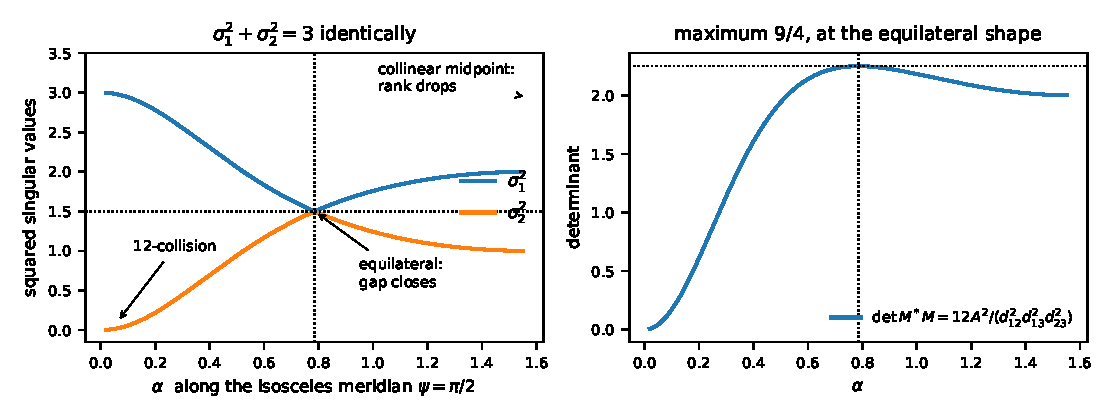
\includegraphics[width=\textwidth]{fig_sheets.pdf}
\caption{Left: the two squared singular values of the shape$\to$distance differential along
the isosceles meridian $\psi=\pi/2$, running from the $12$-collision ($\alpha\to0$) through the
equilateral shape to the collinear midpoint configuration ($\alpha\to\pi/2$). Their sum is $3$ at
every $\alpha$ (Theorem~\ref{thm:shape-sum}); they meet at the equilateral shape, where the gap
closes linearly, and separate toward $(3,0)$, where the rank drops (Theorem~\ref{thm:cone}). Right: the determinant
$12A^2/(d_{12}^2d_{13}^2d_{23}^2)$, maximal and equal to $9/4$ exactly at the equilateral shape
(Theorem~\ref{thm:shape-det}). Both panels are drawn from
\gate{scripts/gates/g01\_shape\_spectrum.py}, not from a separate computation.}
\label{fig:sheets}
\end{figure}

\subsection{Reading the two sheets, and the rigidity that survives}

For equal masses, write $\sigma_\pm^2=\tfrac12\bigl(3\pm\sqrt{9-4\det}\bigr)$. The two sheets
coincide exactly at the equilateral shapes --- the optic points of the birefringent reading ---
and separate on the collinear locus into $(3,0)$. With unequal masses both statements change, and
Theorem~\ref{thm:optic} says how.

\begin{remark}[Rigidity is a choice of variable, not a law to be corrected]\label{rem:rigidity}
For the distance map, $\rho:=\sigma_{\min}^{-2}=2/(3-\sqrt{9-4\det})$ takes the value $2/3$ at the
equilateral shapes and grows like $A^{-2}$ toward the collinear locus. For the squared-distance
map the same definition gives $(\lambda_{\min}/6)^{-2}=\sec^4\vartheta$, since that operator's
$\lambda_{\min}=6\cos^2\vartheta$ (Remark~\ref{rem:twomaps}); this is precisely the three-body
paper's $\rho=\sec^4\vartheta$. The two are not rival values of one quantity: they are
$\sigma_{\min}^{-2}$ for two different operators, and near the collinear locus \emph{both} maps
have $\sigma_2^2\sim\rho_{\mathrm{geom}}^2$ (measured exponent $2.0000$ for each, gate
\gate{g06}, \gate{notes/07\_TWO\_MAPS.md}), so neither exponent is inherited from the
cone-versus-fold distinction. An earlier draft called the fourth power an error inherited from a
mis-stated closing; that was wrong, and the two powers are two definitions.
\end{remark}

\begin{theorem}[The optic points, and what mass breaking does to them]\label{thm:optic}
Let the three masses be arbitrary and let $\sigma_1\ge\sigma_2$ be the singular values of the
distance differential on the shape sphere. Then, for every mass choice we tested, the set of
shapes where $\sigma_1=\sigma_2$ consists of two antipodal points, and at each of them the
degeneracy is a cone. For equal masses the two points are the equilateral shapes and the cone is isotropic
of slope $3$. For unequal masses:
\begin{enumerate}[label=(\roman*)]
\item the two optic points are \emph{displaced} from the equilateral shapes, by a geodesic
distance $=\varepsilon^2/9+O(\varepsilon^3)$ for the family $(1,1,1+\varepsilon)$;
\item the cone at the displaced point is \emph{elliptic}: at $(1,1,2)$ the Hessian of
$\sigma_1^2-\sigma_2^2$ squared has eigenvalues $10.25$ and $13.73$ instead of $(18,18)$;
\item consequently the equilateral shape is \emph{not} an optic point: the gap there is
$3\times$ its distance to the nearest optic point, i.e.\ $\varepsilon^2/3+O(\varepsilon^3)$
for $(1,1,1+\varepsilon)$, and $0.1$ for $(1,1,2)$.
\end{enumerate}
\T/\V\ Gate \gate{g03\_mass\_breaking} (20 assertions), for the mass choices tested: two optic
points in each case, isotropy at equal masses and ellipticity at $(1,1,2)$, displacement exponent $1.995$, displacement
coefficient $0.1096$ against $1/9$, gap-at-equilateral values $0.1$ and $0.196970$ for
$(1,1,2)$ and $(1,2,3)$.
\end{theorem}

\begin{remark}[What mass breaking does, on each map]\label{rem:biaxial}
The three-body paper states that breaking the mass symmetry turns a trivial $+1$ holonomy into
$-1$. On its own operator that is \emph{correct}, and we verify it: for the squared-distance map
the single touching point at equal masses has holonomy $+2\pi$ (sign $+1$), and at masses
$(1,1,1.3)$, $(1,1,2)$ and $(1,2,3)$ it splits into exactly two points, each with holonomy $+1\pi$
(sign $-1$) --- measured at $\alpha$ and $\psi$ listed in \gate{notes/07\_TWO\_MAPS.md}. An
earlier draft of this paper called that prediction wrong; it is not, and the error was ours.
Theorem~\ref{thm:optic} is the corresponding statement for the \emph{distance} map, where the two
touching points are present at equal masses already, are displaced by $\varepsilon^2/9$ and become
an elliptic cone; the two statements describe two operators and do not compete.
\end{remark}

\section{Refraction is conformal geometry, not a new law}\label{sec:refraction}

The corpus states a refraction law $\rho_1\sin^2\theta_1=\rho_2\sin^2\theta_2$ across a
``rigidity interface''. The law is true, and it is Snell's law for a conformal metric; saying so
precisely is the whole content of this section, and it changes the epistemic status of the claim
from a transport law to a consequence of a modelling choice.

\begin{theorem}[Snell from a conformal factor]\label{thm:snell}
Let $g$ be a Riemannian metric on a surface, $R>0$ a function that is $\C^1$ on each side of a
$\C^1$ curve $\shape$ and jumps across it, and $\hat g=R\,g$. Let $\gamma$ be a geodesic of
$\hat g$ crossing $\shape$ transversally at $p$. Then
\begin{equation}\label{eq:snell}
   n_1\sin\theta_1=n_2\sin\theta_2,\qquad\text{equivalently}\qquad
   R_1\sin^2\theta_1=R_2\sin^2\theta_2,
\end{equation}
where $n:=\sqrt R$ and $\theta$ is the angle between $\gamma$ and the normal to $\shape$
measured in the metric $g$.
\T\ (first variation of the $\hat g$-length, with the matching condition at $\shape$).
\end{theorem}

\begin{proof}
A geodesic of $\hat g$ is a critical point of $\hat g$-length against variations supported away
from the endpoints. Taking a variation localised near $p$ and letting its support shrink gives
continuity across $\shape$ of the tangential component of the $\hat g$-unit tangent $u$: for every
vector $\tau$ tangent to $\shape$, $\ip{u}{\tau}_{\hat g}$ is continuous. Let $\tau$ be the
$g$-unit tangent and write $\abs{u}_g=R^{-1/2}$ because $\ip{u}{u}_{\hat g}=R\ip{u}{u}_g=1$.
Then $\ip{u}{\tau}_{\hat g}=R\ip{u}{\tau}_g=R\abs{u}_g\sin\theta=\sqrt R\,\sin\theta$, so
$\sqrt{R_1}\sin\theta_1=\sqrt{R_2}\sin\theta_2$; squaring gives \eqref{eq:snell}.
\end{proof}

\begin{remark}[What is a theorem and what is a hypothesis]\label{rem:snell-grade}
Theorem~\ref{thm:snell} is \T. It is not a statement about any physical transport: it is a
statement about geodesics of a conformal metric. To apply it to a transport one must assert that
admissible paths extremise $\int R\sin^2\theta\,\df s$, or equivalently that the effective metric
is conformal to a reference one with conformal factor $R$. That assertion is a modelling choice,
and it is \Hh\ wherever the corpus makes it. With $\rho$ in the role of $R$ one recovers the
corpus's law and the index $n=\sqrt\rho$; with $\rho=2/(3-\sqrt{9-4\det})$ of
Remark~\ref{rem:rigidity} one gets a specific, falsifiable prediction for the shape sphere,
namely an index that diverges like $1/A$ as collinearity is approached, so that transport across
a near-collinear interface is totally reflected to leading order.
\end{remark}

\begin{remark}[Why the qualification matters]
A ``refraction law'' sounds like a discovered regularity of a system. \eqref{eq:snell} is instead
what one gets for free once one has decided that the medium is conformal with factor $R$ --- the
same content as Fermat's principle, re-expressed. The empirical question is never whether the
law holds, but whether the medium is conformal and with which $R$. That is the question a gate can
answer, and it is the form in which the corpus's interface-refraction protocol should be stated.
\end{remark}

\section{What this paper does not do}\label{sec:scope}

The corpus attaches the framework to cosmology, to measured covariance data, to psychophysics and
to arithmetic. None of that is used above, and none of it is supported by the theorems proved
here. It is graded in one place so that a reader can see what is and is not being claimed.

\paragraph{Covariance data and the transmon/$^{87}$Rb readings.} The corpus reports a reproduction of a
published Chern number ($-0.999$ against $-1.00\pm0.02$) from published Bloch-state tomography.
That is \Dd: a known estimator applied to somebody else's data, reproducing a known value. It
demonstrates that the estimator is implemented correctly. It is not evidence for any distinctive
claim of the framework, because any correct implementation of the same estimator would reproduce
the same number. The distinctive claim --- that the interface refraction test predicts
out-of-sample --- is falsifiable and is the corpus's best methodological idea; it is not tested
here.

\paragraph{The cosmological claim.} A finite-rank truncation $N\sim(M_pR_{\mathrm{univ}})^2$ is
chosen so that a regularised trace-log converges, and an order of magnitude for $\Lambda$ is then
read out of the same regularised sum. That is circular as stated: the answer is carried by the
cutoff. \Hh\ A derivation would need a stability theorem --- that the result is insensitive to
$N$ over a range selected by something other than the desired answer --- and no such theorem is
present. Nothing in \S\S\ref{sec:redistribution}--\ref{sec:shape} depends on it, and the paper
does not use it.

\paragraph{Psychophysical colour spaces.} The reading of colour space as a projector geometry is
an interpretation (\Hh). There is no theorem in it, and the classical Riemannian structure of
colour space \Cc{} does not need one.

\paragraph{The figure-eight and the arithmetic calibration.} The observed invariance of a contour
count along the figure-eight choreography is \V\ in the corpus but is not used here; the arithmetic
calibration (Catalan initial data, band-resolved curvature asymptotics) is \Cc/\V\ and is likewise
not used.

\begin{remark}[Why the scope section is short and blunt]
A paper whose claims can be enumerated is better than one whose claims can only be sampled,
because a reader can check a list. The readings are not withdrawn --- they are placed where
their grade says they belong.
\end{remark}

\section{What would prove this wrong}\label{sec:refute}

Each claim below is paired with the cheapest observation that would falsify it. A test that needs
a new instrument is not a test; none of these does.

\begin{center}
\begin{tabular}{@{}p{0.42\textwidth}p{0.52\textwidth}@{}}
\toprule
claim & what would refute it \\
\midrule
\S\ref{sec:redistribution}: $\Fr$ is traceless and $\Fr=0\iff[\Omega,\PP]=0$ &
a single matrix pair with nonzero trace, or with $\Fr=0$ and $[\Omega,\PP]\neq0$. None exists;
the statements are kernel-checked. Refutation here would mean a bug in Lean. \\
\S\ref{sec:geometry}: $g$ is positive semidefinite &
a projector family with $g(\dot\PP,\dot\PP)<0$ at some point. \\
\S\ref{sec:geometry}: $\abs{\operatorname{Im}Q}\le\sqrt{g_{\mu\mu}g_{\nu\nu}}$ &
a pair of parameters with the ratio exceeding $1$. \\
\S\ref{sec:hierarchy}: rank one gains nothing &
a family with $\norm{\dot P}_{\mathrm{op}}<\norm{\dot v_\perp}$ or
$\norm{\dot P}_F<\sqrt2\norm{\dot v_\perp}$. \\
\S\ref{sec:hierarchy}: cluster projector rate $\norm{\dot A}/\Gap_{\mathrm{ext}}$ &
a family whose cluster projector moves faster than $\norm{\dot A}/\Gap_{\mathrm{ext}}$ (would
refute the constant, not the principle). \\
\S\ref{sec:totals}: $\sum_{i<j}\norm{\nabla d_{ij}}^2=N(N-2)$ &
one configuration of $N$ equal masses with a different total. This is the cheapest test in the
paper: it is a finite computation for any $N$, and a single exception kills it. \\
\S\ref{sec:shape}: $\det M^*M=12A^2/(xyz)$ &
one triangle with a different determinant. Likewise one computation. \\
\S\ref{sec:shape}: the cone is isotropic and linear &
a measurement of the angular dependence of $\sigma_1^2-\sigma_2^2$ near an equilateral shape with
a slope other than $3$, or direction-dependent. \\
\S\ref{sec:shape}: holonomy $-1$ &
a loop around an equilateral shape returning the eigen-line to itself. \\
\S\ref{sec:refraction}: Snell for conformal metrics &
nothing: it is a theorem. What is refutable is the modelling claim that a given physical medium
is conformal with factor $\rho$, and that is refuted by measuring the index directly. \\
\bottomrule
\end{tabular}
\end{center}

\begin{remark}[The asymmetry this paper is trying to fix]
Nine of the ten papers in the corpus say what they explain. One says what would refute it. The
table above is an attempt to make the ratio one to one.
\end{remark}

\section{Open problems}\label{sec:open}

Each problem is stated with the reason it is open, so that a reader can tell a hard problem from
an unattempted one.

\begin{enumerate}[label=\textbf{O\arabic*.},leftmargin=2.4em]
\item \textbf{The angle over a long path.} Theorem~\ref{thm:riesz} settles the derivative bound
(constant $1$, sharp), gives the union-gap form for a single perturbation, and identifies $\pi/2$
as the endpoint value of the angle bound. What is not settled is the \emph{integrated} version:
along a long path with a gap that may shrink, the angle can pass through $\pi/2$ and the count can
change, and no bound is known for the total angular travel in terms of
$\int\norm{\dot A}/\Gap\,\df t$. This is the adiabatic question in a finite-dimensional setting,
and it is open because the derivative bound cannot be integrated past the point where the angle
reaches $\pi/2$. The sketch of what a proof would need is in
\gate{notes/04\_PI\_OVER\_2.md}, whose earlier version stated the problem in the form that
Theorem~\ref{thm:riesz} has now resolved.

\item \textbf{The rank-$k$ $\tan 2\Theta$ bound.} Theorem~\ref{thm:tan2} settles rank one
completely, with an exact constant and an exact sharpness family. The gap to close is
$k\ge2$: given a cluster projector $\PP$ of rank $k$ and an off-diagonal perturbation $V$ whose
spectral sets have disjoint convex hulls, is $\abs{\tan\Theta}\le\delta/d$ for the operator
angle, and with which constant? The rank-one proof does not extend, and the obstruction is
identifiable: its decisive step is $b-a\ge d$, where $b=\ip{Aw}{w}$ ranges over the numerical
range of the compression; for $k\ge2$ one gets such a two-dimensional reduction for each
eigenvector separately, but they do not assemble into a bound on the angular operator
$X$ because the Riccati equation is quadratic, and the elementary trace estimate gives only
$w\norm{X}_F^2-d\norm{X}_F+w\ge0$, which is vacuous when $w<d/2$. What is needed is a solution
theory for $A_+X-XA_-=XBX-B^*$ with an a priori bound on $\norm X$: this is precisely the
machinery of \cite{kmm1,kmm2,kmm3}, which we cite and have not re-derived, and which is where a
proof would begin. A gate sampling the rank-$k$ separated case is described in
\gate{notes/06\_CONVEX\_HULL.md}.

\item \textbf{The optic points, exactly.} Theorem~\ref{thm:optic} locates the two optic points
numerically and gives the displacement law $\varepsilon^2/9+O(\varepsilon^3)$ for one family.
What is missing is a closed form: the displacement is the zero of a two-by-two system whose
entries are algebraic in the masses, so a formula exists and has not been found. The same
question for $N\ge4$ bodies is open and is the natural continuation of \S\ref{sec:shape}.

\item \textbf{A per-shape capacity law.} The sum rule fixes the total; it says nothing about how
the total is distributed. A distribution law would need a statement about the eigenvalues of
$M^*M$ beyond their sum, i.e.\ beyond Theorems~\ref{thm:shape-sum}--\ref{thm:shape-det}. For the
three-body problem the pair $(\operatorname{tr},\det)$ already determines the spectrum, so the
problem is closed there and open from $N=4$ on.

\item \textbf{The square case in general dimension.} When $N=d+1$ the Gram matrix $G=X^\top X$ is
square, its trace-one slice is the shape space, and the transport operator splits into an
eigenvalue sector and an eigenframe sector whose spectra are computable. The corpus states this
with an interlacing theorem; the present paper does not use it, and the statement has not been
re-derived here. It is the natural next theorem, and it is the one most in need of being written
down with its hypotheses explicit.

\item \textbf{The census, quantitatively.} The corpus counts channels and measures plateaus with
a fitted constant $C_0$. Given Theorem~\ref{thm:sumrule}, the natural question is exact: for
$N$ bodies, how many pairwise distances can be resolved to accuracy $\varepsilon$ as the shape
varies over a ball of radius $\delta$? That is a question about the singular values of $M$ and
hence about the constant in a $\sin\theta\ge\varepsilon$ dictionary; it is open, and it is the
form in which ``the price of a direction'' can become a theorem rather than a measurement.
\end{enumerate}

\appendix
\section{The ledger: every claim, its grade, and its evidence}\label{app:ledger}

\begin{center}
\small
\begin{tabular}{@{}p{0.30\textwidth}p{0.10\textwidth}p{0.50\textwidth}@{}}
\toprule
claim & grade & evidence \\
\midrule
Thm~\ref{thm:traceless} $\Tr\Fr=0$ & \T & \lean{GapsAndTotals.redistribution\_traceless} \\
Lem~\ref{lem:blocks} block identities & \T & \lean{redistribution\_block12}, \lean{redistribution\_block21}, \lean{block\_decomposition} \\
Thm~\ref{thm:compat} $\Fr=0\iff[\Omega,\PP]=0$ & \T & \lean{redistribution\_zero\_iff\_commute} \\
Thm~\ref{thm:norm} norm identity & \T & \lean{redistribution\_norm}, \lean{half\_commutator\_norm}, \lean{commutator\_skew} \\
Ex.~\ref{ex:nonnormal} non-normal counterexample & \T/\V & \lean{norm\_needs\_selfadjoint.lean} (must fail) \\
\midrule
Thm~\ref{thm:qgt} $Q$ Hermitian, $g$ PSD & \T & Cauchy--Schwarz on $Z_\mu$; \lean{redistribution\_norm} \\
Rem.~\ref{rem:qgt-correction} $Q^\circ=2g$ is real & \T/\V & \gate{check\_D2\_m7.py}: literal imaginary part $0$ \\
Thm~\ref{thm:curv} closedness, periods & \T/\Cc & Chern--Weil \\
Thm~\ref{thm:bound} curvature bound & \T/\V & \gate{check\_D3\_m1.py} \\
\midrule
Thm~\ref{thm:weyl} Weyl & \Cc & Weyl (1912) \\
Thm~\ref{thm:riesz}(a) finite pair, union gap & \Cc/\V & Davis--Kahan; \gate{g04\_projector\_constant} \\
Thm~\ref{thm:riesz}(b) infinitesimal, constant 1 & \T/\V & Davis--Kahan $+$ limit; \gate{g04} \\
Thm~\ref{thm:riesz}(c) angle, $\pi/2$ at the endpoint & \T/\Cc & $\arcsin$; Albeverio--Motovilov \\
Thm~\ref{thm:tan2} rank one, $\abs{\tan 2\Theta}\le2\delta/d$ & \T/\V & proof above; \gate{g06\_projector\_tan2} \\
Rem.~\ref{rem:tan} off-diagonal $\tan\Theta\le\delta/d$, rank $k$ & \Cc/\V & Motovilov--Selin; \gate{g05\_tan\_theta} \\
Thm~\ref{thm:rankone} rank one, no gain & \T/\V & \gate{g02\_gap\_hierarchy} (a) \\
Thm~\ref{thm:ep} exceptional point & \T/\V & \gate{g02\_gap\_hierarchy} (b) \\
Thm~\ref{thm:winding} winding and sign & \T/\V & \gate{g02\_gap\_hierarchy} (c); \gate{check\_D6\_m8.py} \\
\midrule
Lem~\ref{lem:inertia} inertia identity & \T & expansion \\
Thm~\ref{thm:perpairs} per-pair capacity & \T/\V & \gate{g01\_shape\_spectrum} (g) \\
Thm~\ref{thm:sumrule} sum rule & \T/\V & \gate{g01\_shape\_spectrum} (f) \\
\midrule
Thm~\ref{thm:shape-sum} $\sigma_1^2+\sigma_2^2=3$ & \T/\V & \gate{g01\_shape\_spectrum} (a) \\
Thm~\ref{thm:shape-det} determinant, maximum & \T/\V & \gate{g01\_shape\_spectrum} (b),(c),(h) \\
Thm~\ref{thm:cone} linear isotropic cone & \T/\V & \gate{g01\_shape\_spectrum} (d) \\
Thm~\ref{thm:shape-holonomy} holonomy $-1$ & \T/\V & \gate{g01\_shape\_spectrum} (e) \\
Thm~\ref{thm:optic} the optic points move & \T/\V & \gate{g03\_mass\_breaking} \\
\midrule
Thm~\ref{thm:snell} Snell for conformal metrics & \T & first variation \\
\midrule
physical readings (\S\ref{sec:scope}) & \Dd/\Hh & not used by any theorem \\
\bottomrule
\end{tabular}
\end{center}

\section{Reproduction}\label{app:repro}

\paragraph{Kernel.} The finite algebraic core is \lean{EmergentTransport/GapsAndTotals.lean}
(18 theorems) together with \lean{EmergentTransport/Basic.lean} (11 theorems), checked by
\begin{verbatim}
python3 scripts/verify.py --direct
# OK: 29 theorems, axioms used: ['Classical.choice', 'Quot.sound', 'propext'],
# 6 false controls rejected
\end{verbatim}
The verifier audits the axioms of every named theorem (only the three standard ones are allowed,
which excludes \lean{sorryAx}, project axioms and \lean{native\_decide}), requires six deliberately
false statements to \emph{fail} for a mathematical reason, and records the SHA-256 of every source
file. On a machine where the Mathlib checkout is writable, the same script runs under
\lean{lake env lean} without the flag.

\paragraph{Gates.} Every number in \S\S\ref{sec:redistribution}--\ref{sec:shape} is produced by a
gate that writes JSON:
\begin{verbatim}
python3 scripts/gates/g01_shape_spectrum.py
python3 scripts/gates/g02_gap_hierarchy.py
python3 scripts/gates/g03_mass_breaking.py
python3 scripts/gates/g04_projector_constant.py
python3 scripts/gates/g05_tan_theta.py
python3 scripts/gates/g06_projector_tan2.py
\end{verbatim}
The first has 20 assertions on the shape$\to$distance differential, the second 13 on rank one,
the exceptional point and the sign, the third 20 on the optic points under mass breaking, the fourth 10 on the projector constants and the failure of the constant-1 finite form, the fifth 4 on the off-diagonal $\tan\Theta$ bound, the sixth 12 on the rank-one $\tan 2\Theta$ theorem.
The paper's figures of merit (the closed form of $\det M^*M$, the cone slope, the holonomy, the
per-pair identity) are read from \gate{results/gates/*.json}, never typed by hand.

\paragraph{The swarm records.} The proofs of \S\ref{sec:hierarchy}.2--\S\ref{sec:hierarchy}.5 and of
Theorem~\ref{thm:perpairs} were produced and checked in eight independent directions whose
reports and scripts are in \gate{results/swarm/}, with \gate{README.md} recording what each one
corrected. Three claims in this paper were corrected during that process and the superseded
statements are kept in \gate{notes/02\_PLAN.md}, not deleted.

\section{The classical inputs, stated}\label{app:classical}

For completeness, the two results imported in \S\ref{sec:hierarchy}:

\emph{Weyl.} For self-adjoint $A,A'$ and eigenvalues ordered increasingly,
$\abs{\lambda_i(A')-\lambda_i(A)}\le\norm{A'-A}$. Proof: the min--max characterisation of the
$i$-th eigenvalue makes it $1$-Lipschitz in $A$ in the operator norm.

\emph{Davis--Kahan.} Let a spectral cluster $\shape$ of a self-adjoint $A$ satisfy
$\operatorname{dist}(\shape,\operatorname{spec}A\setminus\shape)\ge\Gap$, and let $\PP,\PP'$ be
the orthogonal projectors onto $\shape$ and onto the corresponding part of the spectrum of
$A'=A+E$. The sine theorem states $\norm{\PP-\PP'}\le\norm{E}/\Gap$, with the denominator the gap
in the \emph{union} of the two spectra --- which is at least $\Gap-\norm{E}$ when $\delta<\Gap/2$.
That is Theorem~\ref{thm:riesz}(a); the derivative form (b) follows by applying it to
$(A(t),A(t+h))$ and letting $h\to0$, and the angle form (c) by monotonicity of $\arcsin$.

\emph{On the constant $\pi/2$.} The estimates in this literature are stated for the
\emph{angle} $\arcsin\norm{\PP-\PP'}$ rather than for $\norm{\PP-\PP'}$ itself, and that is where
$\pi/2$ lives. Albeverio and Motovilov \Cc{} prove a bound of the form
$\arcsin\norm{\PP-\QQ}\le M(\norm{V}/\Gap)$ for $\norm{V}<\Gap/2$, and show that the two subspaces
are guaranteed to be in the acute-angle case only for $\norm{V}<c\,\Gap$ with
$c=0.454169\ldots<1/2$: that is, the angle reaches $\pi/2$ strictly before the stable range ends.
This is exactly the content of Theorem~\ref{thm:riesz}(c) expressed in the literature's
normalisation, and it is the source we attribute the angle form to. For \emph{off-diagonal}
perturbations the angle bound sharpens to Motovilov--Selin's $\tan\Theta\le\delta/d$, which never
reaches $\pi/2$; see Remark~\ref{rem:tan}, whose transcription of that bound is checked by gate
\gate{g05\_tan\_theta}.

We could \emph{not} verify that Kato's book states the constant $\pi/2$. The zbMATH review of the
1966 edition (Zbl 0148.12601) summarises Chapter II as finite-dimensional analytic perturbation
theory with perturbation series for eigenprojectors, a reduction method for semisimple
eigenvalues, and estimates of convergence radii --- without naming a constant --- and the sections
themselves were not available to us. The attribution to Kato is therefore dropped, not as a
disagreement but for want of evidence; the mathematics used in \S\ref{sec:hierarchy} is
Theorem~\ref{thm:riesz}, resting on Davis--Kahan for the finite-pair bound, on the limit for the
derivative, and on the elementary inequality $\arcsin x\le(\pi/2)x$ for the angle.


\begin{thebibliography}{99}
\bibitem{weyl} H.~Weyl, \emph{Das asymptotische Verteilungsgesetz der Eigenwerte linearer partieller Differentialgleichungen}, Math. Ann. \textbf{71} (1912), 441--479.
\bibitem{kato} T.~Kato, \emph{Perturbation Theory for Linear Operators}, Springer, 1966. Cited for analytic perturbation theory in general; the constant $\pi/2$ discussed in the literature on his name is not used here (see Appendix~\ref{app:classical}).
\bibitem{dk} C.~Davis and W.~M.~Kahan, \emph{The rotation of eigenvectors by a perturbation III}, SIAM J.\ Numer.\ Anal.\ \textbf{7} (1970), 1--46.
\bibitem{berry} M.~V.~Berry, \emph{Quantal phase factors accompanying adiabatic changes}, Proc.\ Roy.\ Soc.\ London A \textbf{392} (1984), 45--57.
\bibitem{pv} J.~P.~Provost and G.~Vallee, \emph{Riemannian structure on manifolds of quantum states}, Comm.\ Math.\ Phys.\ \textbf{76} (1980), 289--301.
\bibitem{iqgt} J.~Beasley, \emph{Intrinsic Quantum Geometric Tensor on the Grassmannian and Spectral Lower Bounds on Dissipation}, 13 October 2026, DOI 10.5281/zenodo.23351266.
\bibitem{corpus3b} J.~Beasley, \emph{The Three-Body Problem, Operator-First: A Complete Spectral Anatomy of Relational Transport}, 24 August 2026, DOI 10.5281/zenodo.22080702.
\bibitem{kmm1} V.~Kostrykin, K.~A.~Makarov and A.~K.~Motovilov, \emph{On the existence of solutions to the operator Riccati equation and the $\tan\Theta$ theorem}, Integral Equations Oper.\ Theory \textbf{51} (2005), 121--140; arXiv:math.SP/0210032; Zbl 1089.47015.
\bibitem{kmm2} V.~Kostrykin, K.~A.~Makarov and A.~K.~Motovilov, \emph{A generalization of the $\tan 2\Theta$ theorem}, in: Current Trends in Operator Theory and its Applications, Oper.\ Theory Adv.\ Appl.\ \textbf{149} (2004), 349--372; arXiv:math.SP/0302020; Zbl 1084.47002.
\bibitem{kmm3} V.~Kostrykin, K.~A.~Makarov and A.~K.~Motovilov, \emph{Perturbation of spectra and spectral subspaces}, Trans.\ Amer.\ Math.\ Soc.\ \textbf{359} (2007), 77--89; arXiv:math.SP/0306025; Zbl 1115.47014.
\bibitem{am} S. Albeverio and A.~K. Motovilov, \emph{Sharpening the norm bound in the subspace perturbation theory}, Complex Anal.\ Oper.\ Theory \textbf{7} (2013), 1389--1416; arXiv:1112.0149; Zbl 1288.47006.
\bibitem{ms} A.~K. Motovilov and A.~V. Selin, \emph{Some sharp norm estimates in the subspace perturbation problem}, Integral Equations Oper.\ Theory \textbf{56} (2006), 511--542; arXiv:math/0409558; Zbl 1121.47007.
\bibitem{chern} S.-S.~Chern, \emph{Characteristic classes of Hermitian manifolds}, Ann.\ of Math.\ \textbf{47} (1946), 85--121.
\bibitem{kendall} D.~G.~Kendall, \emph{Shape manifolds, procrustean metrics, and complex projective spaces}, Bull.\ London Math.\ Soc.\ \textbf{16} (1984), 81--121.
\bibitem{corpus} J.~Beasley, the operator-first transport series, 2026, of which this paper is a part; the editions used for the inventory and review are listed in \texttt{notes/00\_INVENTORY.md}. The paper that this one replaces as the framework's statement is \emph{Intrinsic Emergent Transport Geometry}, DOI \texttt{10.5281/zenodo.21089303}.
\end{thebibliography}


\end{document}
